% vim: set spell spelllang=en tw=100 et sw=4 sts=4 foldmethod=marker foldmarker={{{,}}} :

\documentclass[aspectratio=169,compress,10pt]{beamer}

\usepackage{tikz}
\usepackage{xcolor}
\usepackage{complexity}
\usepackage{hyperref}
\usepackage{microtype}
\usepackage{amsmath}                   % \operatorname
\usepackage{amsfonts}                  % \mathcal
\usepackage{amssymb}                   % \nexists
\usepackage[vlined]{algorithm2e} % algorithms
\usepackage{centernot}
\usepackage{listings}
\usepackage{csquotes}
\usepackage{fancyvrb}
\usepackage{bussproofs}
\usepackage{multicol}
\usepackage{booktabs}
\usepackage{mathtools}
\usepackage{pifont}
\usepackage{marvosym}
\usepackage{cancel}

\usefonttheme{professionalfonts}

\usetikzlibrary{shapes, arrows, shadows, calc, positioning, fit}
\usetikzlibrary{decorations.pathreplacing, decorations.pathmorphing, shapes.misc}
\usetikzlibrary{tikzmark, backgrounds}
\usetikzlibrary{trees, overlay-beamer-styles}

\definecolor{uofguniversityblue}{rgb}{0, 0.219608, 0.396078}
\definecolor{uofgheather}{rgb}{0.356863, 0.32549, 0.490196}
\definecolor{uofgaquamarine}{rgb}{0.603922, 0.72549, 0.678431}
\definecolor{uofgslate}{rgb}{0.309804, 0.34902, 0.380392}
\definecolor{uofgrose}{rgb}{0.823529, 0.470588, 0.709804}
\definecolor{uofgmocha}{rgb}{0.709804, 0.564706, 0.47451}
\definecolor{uofgsandstone}{rgb}{0.321569, 0.278431, 0.231373}
\definecolor{uofgforest}{rgb}{0, 0.2, 0.129412}
\definecolor{uofglawn}{rgb}{0.517647, 0.741176, 0}
\definecolor{uofgcobalt}{rgb}{0, 0.615686, 0.92549}
\definecolor{uofgturquoise}{rgb}{0, 0.709804, 0.819608}
\definecolor{uofgsunshine}{rgb}{1.0, 0.862745, 0.211765}
\definecolor{uofgpumpkin}{rgb}{1.0, 0.72549, 0.282353}
\definecolor{uofgthistle}{rgb}{0.584314, 0.070588, 0.447059}
\definecolor{uofgrust}{rgb}{0.603922, 0.227451, 0.023529}
\definecolor{uofgburgundy}{rgb}{0.490196, 0.133333, 0.223529}
\definecolor{uofgpillarbox}{rgb}{0.701961, 0.047059, 0}
\definecolor{uofglavendar}{rgb}{0.356863, 0.301961, 0.580392}

% {{{ theme things
\useoutertheme[footline=authortitle]{miniframes}
\useinnertheme{rectangles}

\setbeamerfont{block title}{size={}}
\setbeamerfont{title}{size=\large,series=\bfseries}
\setbeamerfont{section title}{size=\large,series=\mdseries}
\setbeamerfont{author}{size=\normalsize,series=\mdseries}
\setbeamercolor*{structure}{fg=uofguniversityblue}
\setbeamercolor*{palette primary}{use=structure,fg=black,bg=white}
\setbeamercolor*{palette secondary}{use=structure,fg=white,bg=uofgcobalt}
\setbeamercolor*{palette tertiary}{use=structure,fg=white,bg=uofguniversityblue}
\setbeamercolor*{palette quaternary}{fg=white,bg=black}
\setbeamercolor{block body}{bg=structure!10}
\setbeamercolor{block title}{bg=structure,fg=white}
\setbeamertemplate{blocks}[rounded]
\setbeamercolor*{titlelike}{parent=palette primary}

\beamertemplatenavigationsymbolsempty
\setbeamersize{text margin left=0.5cm}
\setbeamersize{text margin right=0.5cm}

\setbeamertemplate{title page}
{
    \begin{tikzpicture}[remember picture, overlay]
        \node at (current page.north west) {
            \begin{tikzpicture}[remember picture, overlay]
                \fill [fill=uofguniversityblue, anchor=north west] (0, 0) rectangle (\paperwidth, -2.6cm);
            \end{tikzpicture}
        };

        \node (logo) [anchor=north east, shift={(-0.8cm,-0.2cm)}] at (current page.north east) {
            
\includegraphics[keepaspectratio=true,scale=0.5]{../../images/UoG_keyline.pdf}
        };

        \node (logo2) [anchor=north, below=0.2cm of logo.south] {
            
\includegraphics[keepaspectratio=true,scale=0.1]{../../images/RAEngWhite.pdf}
        };

        \coordinate (logos) at ($(logo.south)!0.5!(logo2.north)$);

        \node [anchor=west, xshift=0.8cm] at (current page.west |- logos) {
            \begin{minipage}{0.65\paperwidth}\raggedright
                {\usebeamerfont{title}\usebeamercolor[white]{}\inserttitle}\\[0.2cm]
                {\usebeamerfont{author}\usebeamercolor[white]{}\insertauthor}
            \end{minipage}
        };
    \end{tikzpicture}
}

\setbeamertemplate{section page}
{
    \begin{centering}
        \begin{beamercolorbox}[sep=12pt,center]{part title}
            \usebeamerfont{section title}\insertsection\par
        \end{beamercolorbox}
    \end{centering}
}

\newcommand{\frameofframes}{/}
\newcommand{\setframeofframes}[1]{\renewcommand{\frameofframes}{#1}}

\makeatletter
\setbeamertemplate{footline}
{%
    \begin{beamercolorbox}[colsep=1.5pt]{upper separation line foot}
    \end{beamercolorbox}
    \begin{beamercolorbox}[ht=2.5ex,dp=1.125ex,%
        leftskip=.3cm,rightskip=.3cm plus1fil]{title in head/foot}%
        {\usebeamerfont{title in head/foot}\insertshorttitle}%
        \hspace{0.22\textwidth}%
        {\usebeamerfont{author in head/foot}\insertshortauthor}%
        \hfill%
        {\usebeamerfont{frame number}\usebeamercolor[fg]{frame number}\insertframenumber~\frameofframes~\inserttotalframenumber}
    \end{beamercolorbox}%
    \begin{beamercolorbox}[colsep=1.5pt]{lower separation line foot}
    \end{beamercolorbox}
}

\makeatletter
\setbeamertemplate{mini frame}
{%
  \begin{pgfpicture}{0pt}{0pt}{.04cm}{.04cm}
    \pgfpathcircle{\pgfpoint{0.04cm}{0.04cm}}{0.04cm}
    \pgfusepath{fill,stroke}
  \end{pgfpicture}%
}
\setbeamertemplate{mini frame in current subsection}
{%
  \begin{pgfpicture}{0pt}{0pt}{.04cm}{.04cm}
    \pgfpathcircle{\pgfpoint{0.04cm}{0.04cm}}{0.04cm}
    \pgfsetfillcolor{section in head/foot.bg}
    \pgfusepath{fill,stroke}
  \end{pgfpicture}%
}

\setbeamersize{mini frame size=0.10cm, mini frame offset=0.06cm}
\makeatother

\makeatletter
\newenvironment{nearlyplainframe}[2][]{
    \def\beamer@entrycode{\vspace*{-\headheight}\vspace*{3pt}}
    \setbeamertemplate{headline}
    {%
        \begin{beamercolorbox}[colsep=1.5pt]{upper separation line head}
        \end{beamercolorbox}
        \begin{beamercolorbox}[ht=0.5ex,dp=0.125ex,%
            leftskip=.3cm,rightskip=.3cm plus1fil]{title in head/foot}%
        \end{beamercolorbox}%
        \begin{beamercolorbox}[ht=0.5ex,dp=0.125ex,%
            leftskip=.3cm,rightskip=.3cm plus1fil]{author in head/foot}%
        \end{beamercolorbox}%
        \begin{beamercolorbox}[colsep=1.5pt]{lower separation line head}
        \end{beamercolorbox}
        \vspace*{\headheight}
    }

    \setbeamertemplate{footline}
    {%
        \begin{beamercolorbox}[colsep=1.5pt]{upper separation line foot}
        \end{beamercolorbox}
        \begin{beamercolorbox}[ht=0.5ex,dp=0.125ex,%
            leftskip=.3cm,rightskip=.3cm plus1fil]{author in head/foot}%
        \end{beamercolorbox}%
        \begin{beamercolorbox}[ht=0.5ex,dp=0.125ex,%
            leftskip=.3cm,rightskip=.3cm plus1fil]{title in head/foot}%
        \end{beamercolorbox}%
        \begin{beamercolorbox}[colsep=1.5pt]{lower separation line foot}
        \end{beamercolorbox}
    }

    \begin{frame}[#1]{#2}
    }{
    \end{frame}
}
\makeatother

% }}}

\author{Matthew McIlree and Ciaran McCreesh}
\title{Proof Logging for Smart Extensional Constraints}

\begin{document}

{
    \usebackgroundtemplate{
        \tikz[overlay, remember picture]
        \node[at=(current page.south), anchor=south, inner sep=0pt, yshift=-1.4cm]{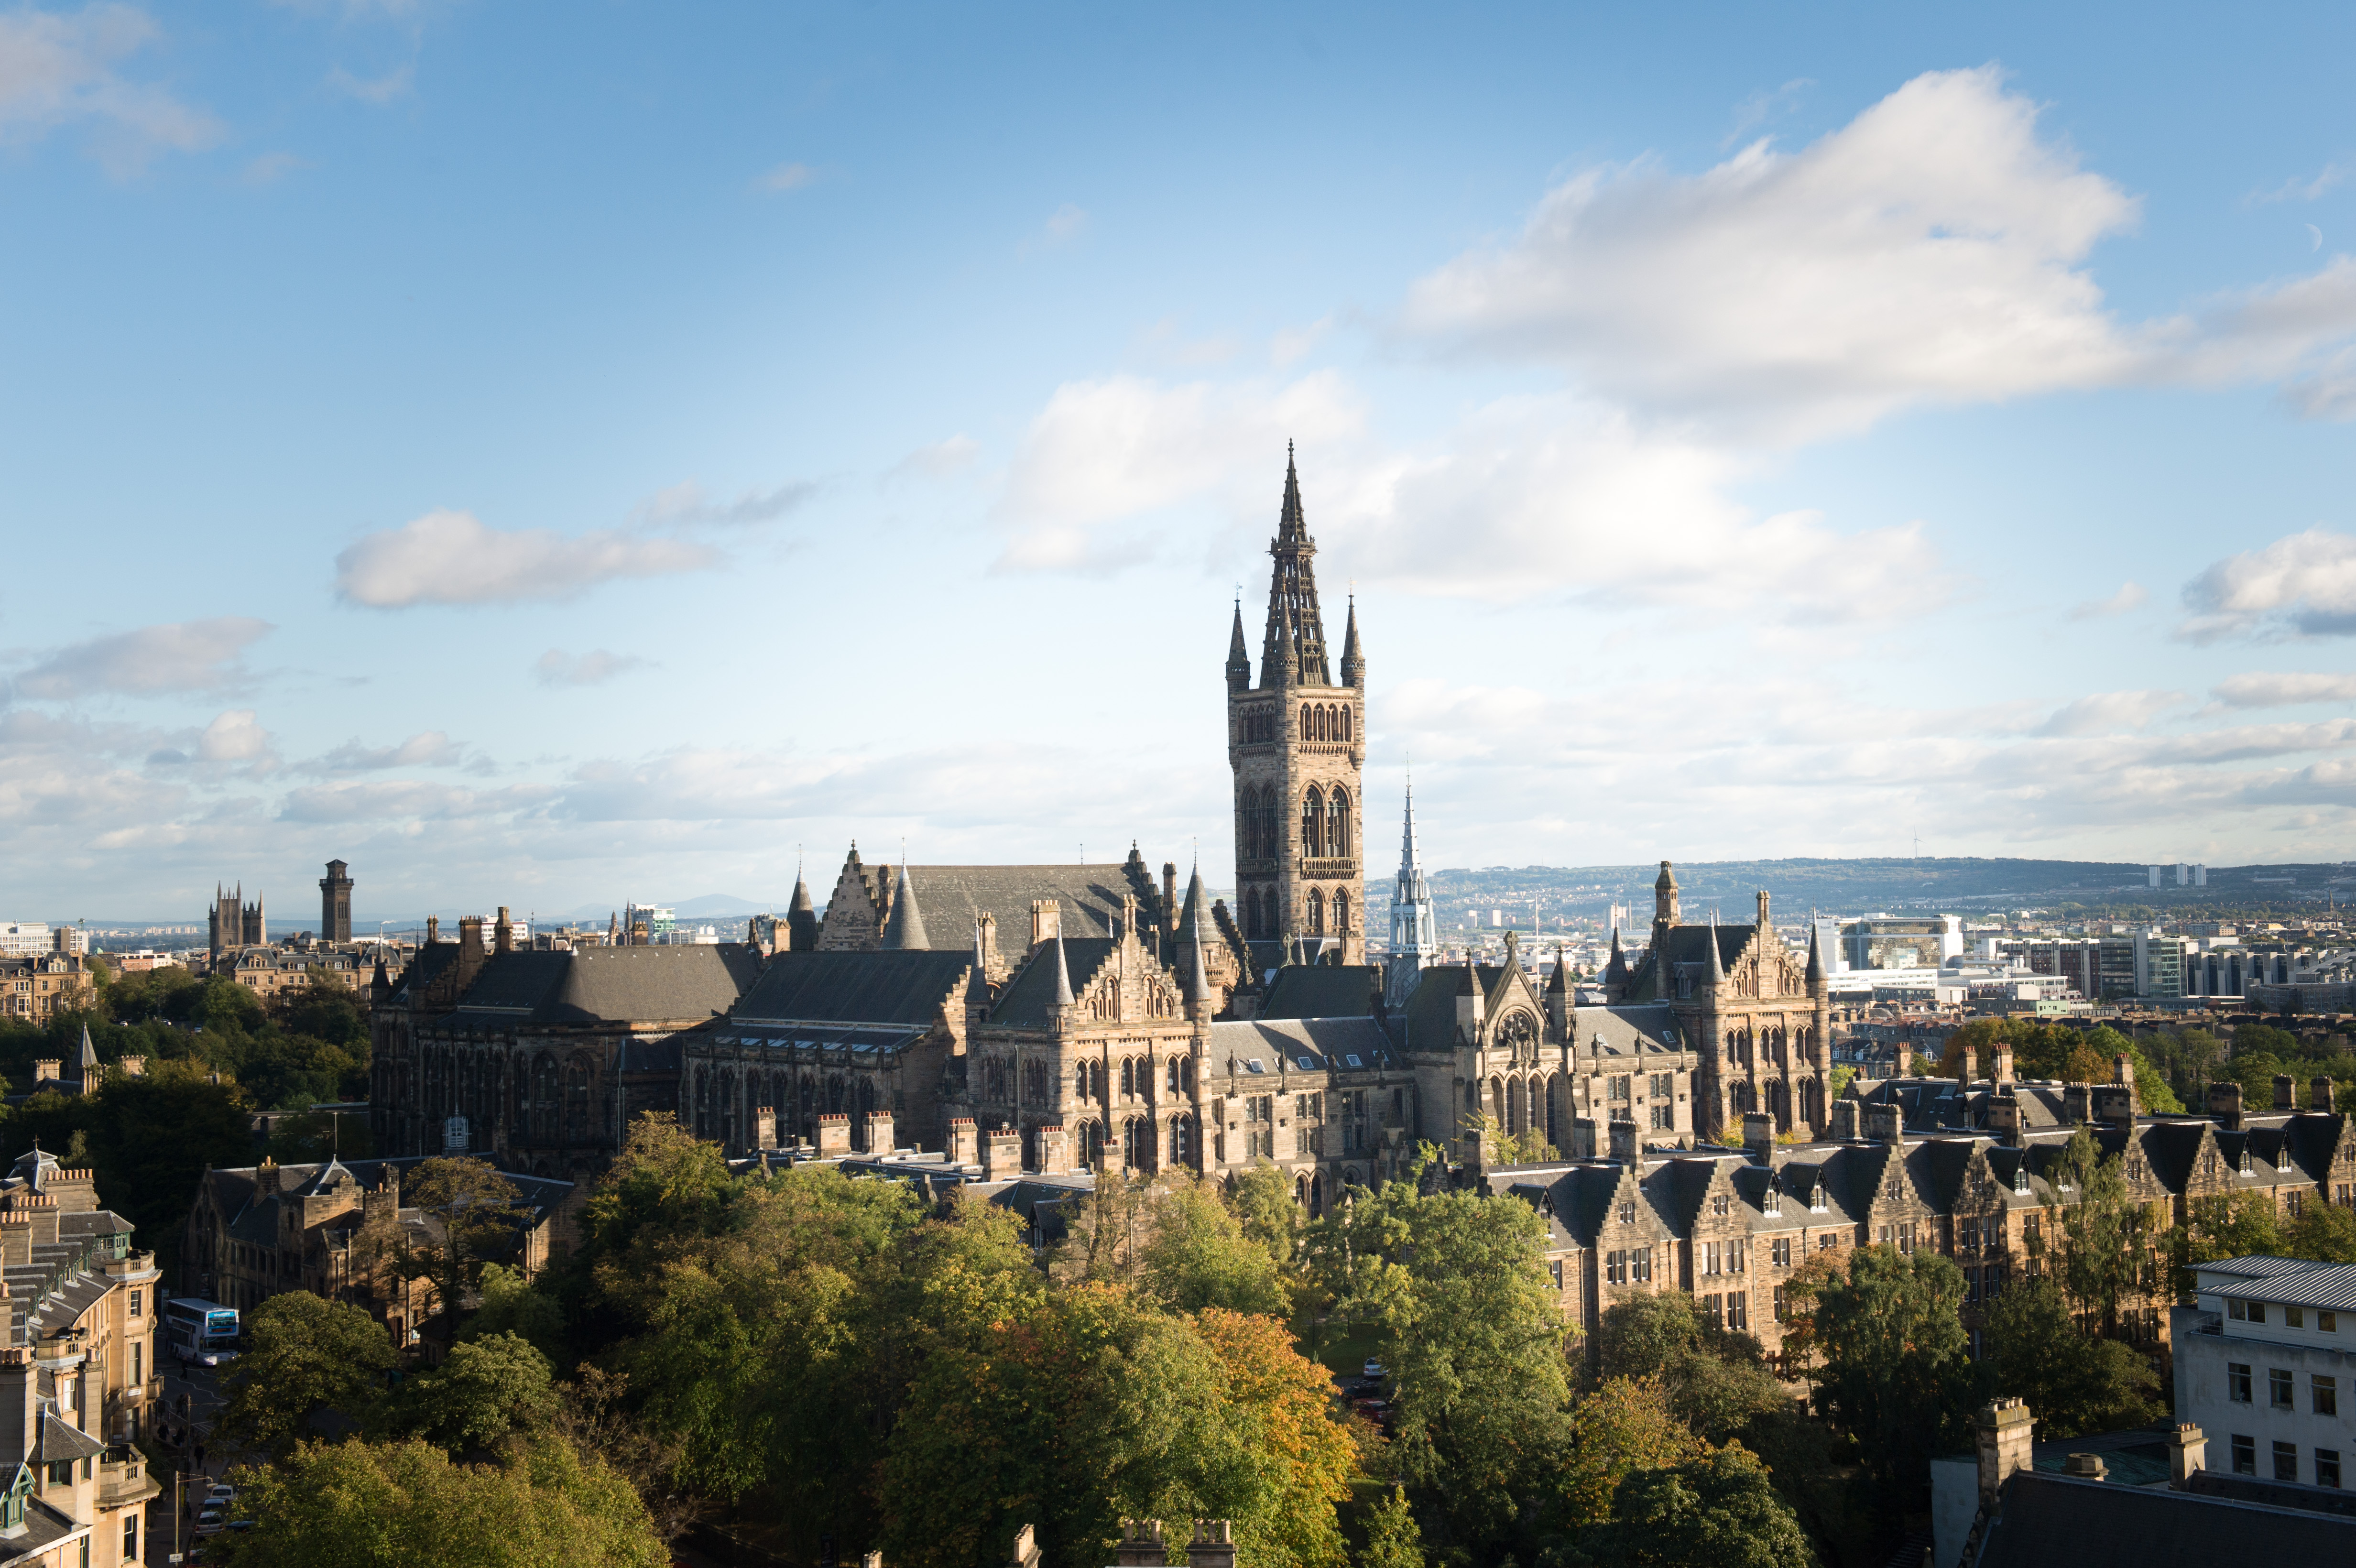
\includegraphics[keepaspectratio=true, width=\paperwidth]{../../images/background.jpg}};
    }
    \begin{frame}[plain,noframenumbering]
        \titlepage
    \end{frame}
}

\section{Proof Logging}

\begin{frame}{The Slide That Keeps Getting Me Into Trouble}
    2021 MiniZinc challenge: for 1.28\% of instances, wrong solutions were claimed.
    \\
    \begin{itemize}
        \item False claims of unsatisfiability.
        \item False claims of optimality.
        \item Infeasible solutions produced.
        \item Not limited to a single solver, problem, or constraint.
        \item Not even consistent---same solver on same hardware and same instance can give
            different results on different runs.
    \end{itemize}
\end{frame}

\begin{frame}{Proof Logging}
    \vspace*{-1.0em}
    \begin{center}
        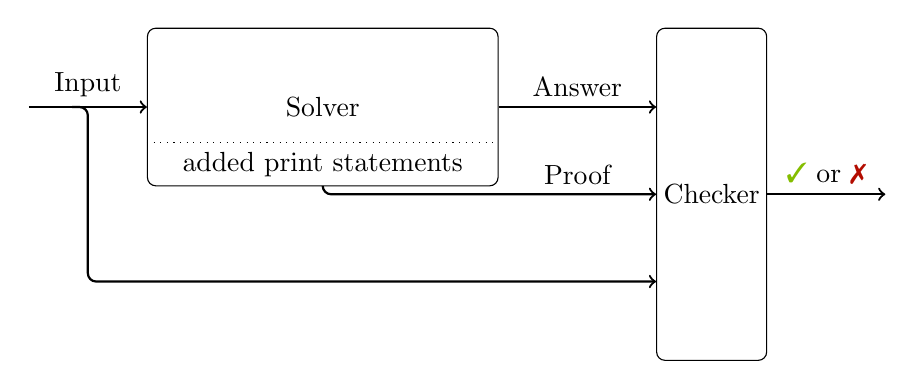
\begin{tikzpicture}
            \node (solver) [inner xsep=5em, inner ysep=2.5em, draw, rounded corners=3pt] { Solver };

            \node (checker) [right=2cm of solver.north east, anchor=north west, inner xsep=0.25em, draw, rounded corners=3pt, minimum height=12em, visible on=<3->] { Checker };

            \node (print) [anchor=south, above=0cm of solver.south, visible on=<2->] { added print statements };
            \draw [dotted, visible on=<2->] (solver.west|-print.north) -- (solver.east|-print.north);

            \draw [->, thick] (solver.east) -- (solver.east -| checker.west)
                coordinate [midway] (solutionmid) node [above, midway] { Answer };

            \draw [->, thick, rounded corners=3pt, visible on=<2->] (solver.south) -- (solver.south |- checker.west)
                -- (checker.west) coordinate [midway] (proofmid);

            \coordinate (prooflabel) at (proofmid-|solutionmid);
            \node [above=0cm of prooflabel, visible on=<2->] { Proof };

            \coordinate [right=1.5cm of checker.east] (verified);
            \draw [->, thick, visible on=<4->] (checker.east) -- (verified) node [above, midway] { \textcolor{uofglawn}{\ding{51}} or \textcolor{uofgpillarbox}{\ding{55}} };

            \coordinate [left=1.5cm of solver.west] (input);
            \draw [->, thick] (input) -- (solver.west) coordinate [midway] (inputmid) node [above, midway] { Input };

            \coordinate (checkerbotleft) at ($(checker.west)+($(checker.west)-(solver.east-|checker.west)$)$);

            \draw [->, thick, rounded corners=3pt, visible on=<3->] ($(inputmid)+(-0.2,0)$) -- (inputmid) -- (inputmid |- checkerbotleft) -- (checkerbotleft);
        \end{tikzpicture}
      \end{center}
    \vspace*{-0.7em}
  \begin{enumerate}
  \item<1->
    Run solver on problem input.
  \item<2->
    Solver also prints out a proof as part of its output.
  \item<3->
    Feed input + solution + proof to proof checker.
  \item<4->
    Verify that proof checker says solution is correct.
  \end{enumerate}
\end{frame}

\begin{frame}{Opinionated Requirements For This To Work}
    Established technology for Boolean Satisfiability (SAT), but severe theoretical
        and practical difficulties for richer reasoning paradigms\ldots \pause
    \begin{enumerate}
        \item Must efficiently work with what solvers actually do, not idealised algorithms. \pause
        \item No need for a new proof format for every new propagator or solver.
            \begin{itemize}
                \item Constraint programming has 423 different global constraints, many of which
                    have several different propagators.
                \item Some propagators are buggy, and at least one has faulty theory behind it\ldots
            \end{itemize} \pause
        \item Proof format must still be simple and well-founded.
            \begin{itemize}
                \item Need to be able to trust the verifier.
                \item Interactions between features can be subtle: even deletions aren't that easy
                    to get right.
            \end{itemize}
    \end{enumerate}
\end{frame}

\begin{frame}{The VeriPB Proof System}
    \begin{center}
        \url{https://www.bartbogaerts.eu/talks/veripb-tutorial-series/}
    \end{center}
    \bigskip
    \begin{itemize}
        \item We can do everything we want with a simple proof format built upon cutting planes
            reasoning with strengthening for pseudo-Boolean problems.
        \item Used for state of the art solvers for subgraph problems, MaxSAT, advanced SAT
            techniques like symmetry breaking and XOR reasoning, MIP preprocessing, \ldots
        \item Key idea: justifying reasoning can use a different language to solving. We are
            \emph{not} writing pseudo-Boolean solvers!
    \end{itemize}
\end{frame}

\begin{frame}{Proofs for Constraint Programming}
    \begin{center}
        \url{https://github.com/ciaranm/glasgow-constraint-solver}
    \end{center}
    \bigskip
    \begin{itemize}
        \item Proofs describe a backtrack search tree, together with extra justifications
            for propagations.
        \item Anything the solver knows must be reflected in the proof log.
        \item Like lazy clause generation, except constraints must be justified rather
            than asserted.
        \item Must work out how to do this for every propagation algorithm.
    \end{itemize}
\end{frame}

\section{Table Constraints}

\begin{frame}{Classical Table Constraints}
    \begin{equation*}
        (A, B, C) \in [(1, 2, 3), (1, 3, 4), (2, 2, 5)]
    \end{equation*}

    \begin{itemize}
        \item A list of possible solutions to the constraint.
        \item A bit like DNF.
    \end{itemize}
\end{frame}

\begin{frame}{Smart Table Constraints}
    \begin{align*}
        (&A, &&B, &&C&)& \in [\\
        (&\ge1, &&2, &&*&)&, \\
        (&=B, &&*, &&\ne2&)&, \\
        (&=C+1, &&\in\{2,4,6\}, &&*&)&]
    \end{align*}

    \begin{itemize}
        \item Allows wildcards and certain complex expressions.
        \item Exponentially smaller representations for some constraints.
        \item Still has an efficient domain-consistent propagator.
    \end{itemize}
\end{frame}

\section{Regular Constraints}

\begin{frame}{Regular Language Membership Constraints}
    \begin{equation*}
        (A, B, C, D, E) ~\operatorname{matches}~ (1{*}[23]4{*})|([23]{*}[45]{*}1{*})
    \end{equation*}
    \begin{itemize}
        \item A different compact representation of all solutions for a given set of
            variables.
        \item Has an efficient incremental domain-consistent propagator.
    \end{itemize}
\end{frame}

\section{This Work}

\begin{frame}{This Work}
    \begin{itemize}
        \item Can efficiently and practically certify every propagation carried out by
            a domain-consistent propagator for smart table and for regular.
            \begin{itemize}
                \item Key idea: propagators \emph{detect} inconsistencies in a clever
                    efficient way, but once detected, can be \emph{justified} similar
                    to lookahead.
            \end{itemize}
        \item Proofs use only information already available to the solver, and are
            `worst case the same length as' the `amount of work carried out by the propagator'.
            \begin{itemize}
                \item Even for incremental propagators!
            \end{itemize}
        \item Corollary: efficient proof logging for many more constraints, such as Lex,
            AtMostOne, NotAllEqual, Stretch, Geost, DiffN, \ldots
    \end{itemize}
\end{frame}

\begin{frame}{Join The Proof Logging Revolution}
    \begin{center}
        \url{https://www.bartbogaerts.eu/talks/veripb-tutorial-series/}
    \end{center}

    \bigskip

    \begin{center}
        \url{https://gitlab.com/MIAOresearch/software/VeriPB}
    \end{center}

    \bigskip

    \begin{center}
        \url{https://github.com/ciaranm/glasgow-constraint-solver}
    \end{center}
\end{frame}

{
    \usebackgroundtemplate{
        \tikz[overlay, remember picture]
        \node[at=(current page.south), anchor=south, yshift=-1cm, inner sep=0pt]{\includegraphics[keepaspectratio=true, width=\paperwidth]{../../images/background2.jpg}};
    }

    \begin{frame}[plain,noframenumbering]
        \begin{tikzpicture}[remember picture, overlay]
            \node at (current page.north west) {
                \begin{tikzpicture}[remember picture, overlay]
                    \fill [fill=uofguniversityblue, anchor=north west] (0, 0) rectangle (\paperwidth, -2.8cm);
                \end{tikzpicture}
            };

            \node (logo) [anchor=north east, shift={(-0.8cm,-0.2cm)}] at (current page.north east) {
                
\includegraphics[keepaspectratio=true,scale=0.5]{../../images/UoG_keyline.pdf}
            };

            \node (logo2) [anchor=north, below=0.2cm of logo.south] {
                
\includegraphics[keepaspectratio=true,scale=0.1]{../../images/RAEngWhite.pdf}
            };

            \coordinate (logos) at ($(logo.south)!0.5!(logo2.north)$);

            \node [anchor=west, xshift=0.8cm] at (current page.west |- logos) {
                \begin{minipage}{0.60\paperwidth}\raggedright
                    \textcolor{white}{\url{https://ciaranm.github.io/}} \\[0.3cm]
                    \textcolor{white}{\href{mailto:ciaran.mccreesh@glasgow.ac.uk}{\nolinkurl{ciaran.mccreesh@glasgow.ac.uk}}}
                \end{minipage}
            };
        \end{tikzpicture}
    \end{frame}
}

\end{document}

